Android Studio ist eine Entwicklungsumgebung für Android auf der Basis von IntelliJ.
IntelliJ ist eine bereits bestehende Entwicklungsumgebung für Java und Android.
Im Grunde wurde Android Studio mit der Hinsicht auf Applikationsentwicklung für das Android-Betriebssystem erstellt. Es beinhaltet von Haus aus notwendige, aber auch arbeitserleichternde Komponenten, wie
einen Gradle-Compiler (notwendig) oder einen Android-Emulator (erleichtert das Testen der App auf einem Computer).\\

Gradle ist ein Programm, das beim Kompilieren als erstes ausgeführt wird. Gradle steuert und übernimmt teilweise Aufgaben von den Java Compilern.
Gradle ist hauptsächlich ein Zusammenträger von zusätzlichen Paketen und Dateien, die für das Kompilieren erforderlich sind. Dabei werden Dateien und Bibliotheken aus dem Internet heruntergeladen,
die man zu der Quellenliste hinzugefügt hat. Dies erleichtert das Hinzufügen von Bibliotheken wie z.B. einer Bibliothek zum Herunterladen und Anzeigen von Bildern, da man nur die Download Adresse angeben muss
und sich nicht mehr um das Einbinden kümmern muss.

\begin{figure}[htbp]
 \centering
    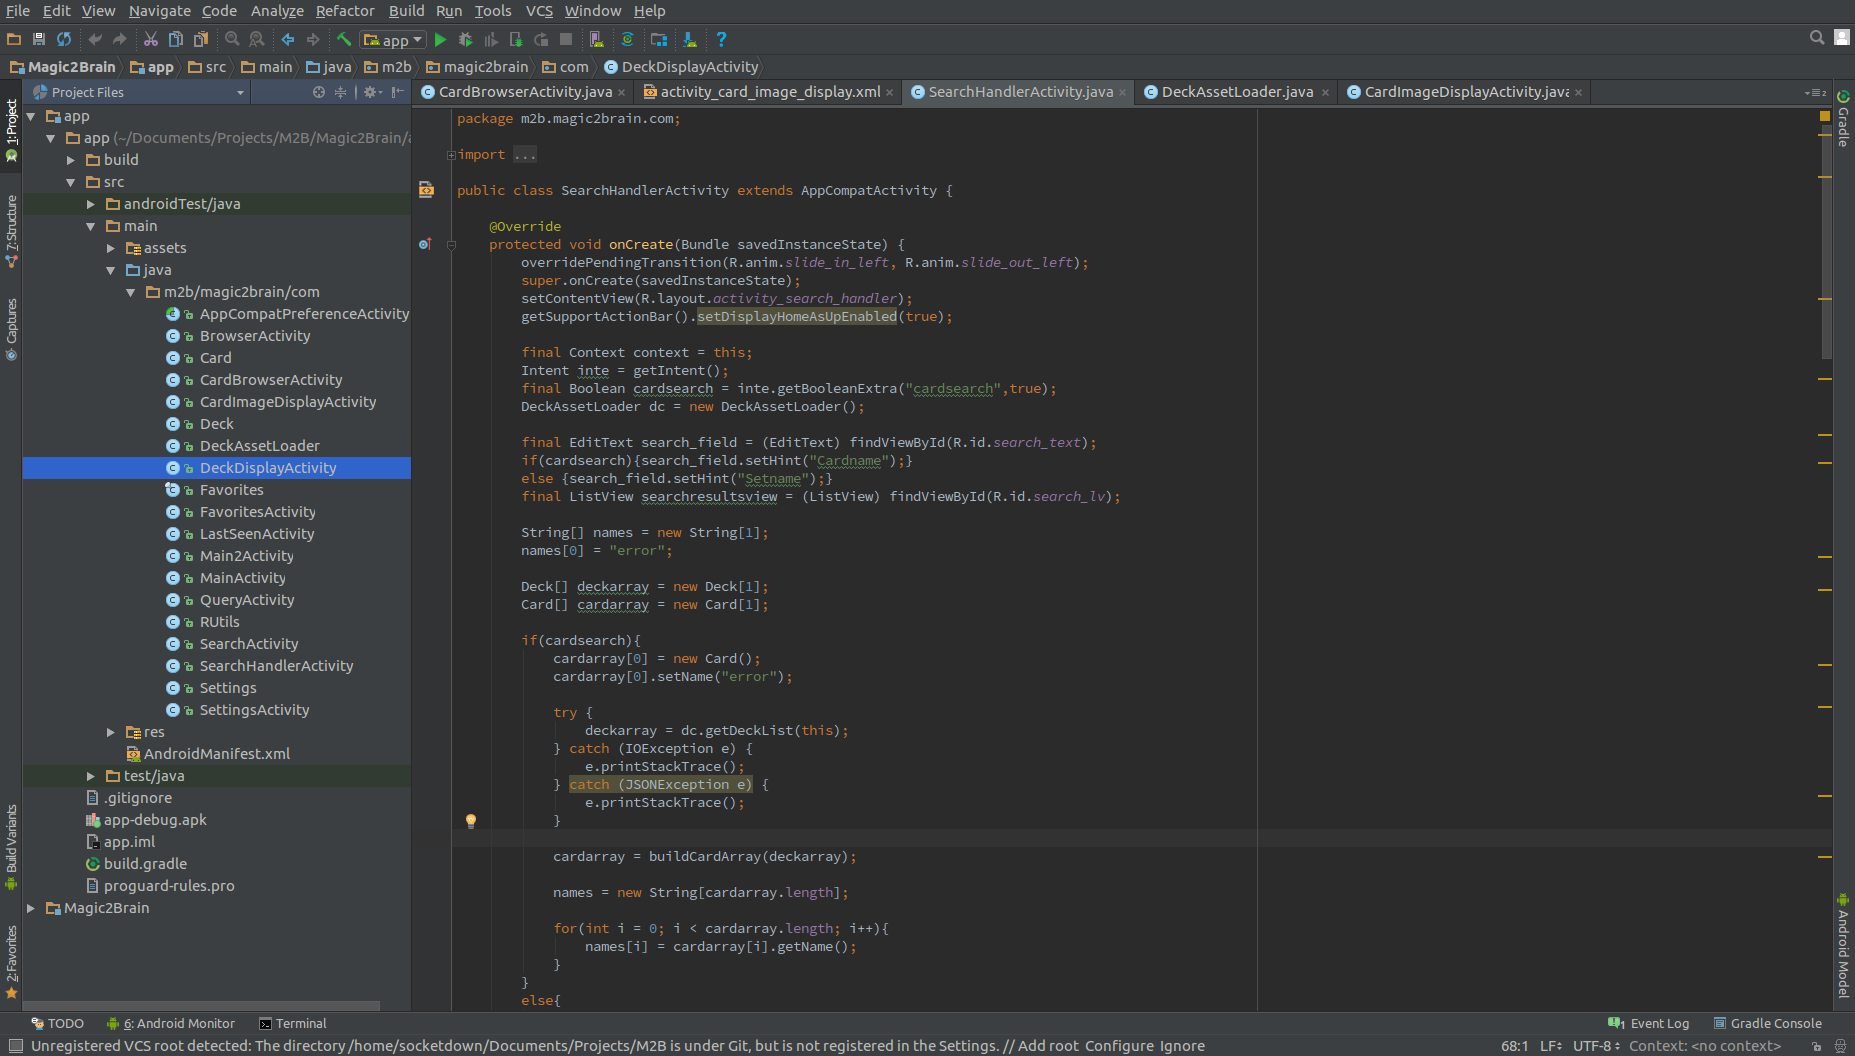
\includegraphics[width=1\textwidth]{AndroidStudio_GUI.png}
 \caption{Android Studio Benutzeroberfläche \cite{ASGUI}}
 \label{fig:Android Studio GUI}
\end{figure}
Die grafische Benutzeroberfläche ist das Wichtigste an einer IDE. Sie erleichtert dem Entwickler die Navigation durch seinen Code in Form von Color-Highlighting (rechts) und Dateibrowser (links).
Die Toolbar von Android Studio (oben) ist mit wichtigen Shortcuts, wie z.B. Kompilierung starten oder Emulator starten gefüllt.
Der Editor von Android Studio erlaubt eine automatische Vervollständigung mit Alt+Enter. Mitunter sind auch schon fertige Vorlagen für Activities in Android Studio verfügbar, die auf Knopfdruck in das Projekt kopiert werden und gleichzeitig für die Kompilierung registriert werden. Activities sind Java-Klassen, die der Benutzer letztendlich braucht. Der Dateibrowser erlaubt es zwischen Quellcode-Dateien zu wechseln und diese zur Bearbeitung zu öffnen. Zusätzlich sind Funktionen zum importieren von Dateien oder Assets vorhanden. Mit Assets sind hier nicht Immobilien oder Vermögen gemeint, sondern Dateien, die von der App benötigt werden um richtig zu funktionieren. Dazu gehören Bilder, Musikdateien und generell alles was kein Quellcode ist. Der IDE kann man auch Plugins hinzufügen. Plugins sind kleine Programmerweiterungen, welche dazugeladen werden können. Bei der Entwicklung von Magic2Brain ist das Plugin "Asset Studio" besonders nützlich gewesen, da man mit ihm Icons nicht nur zu den Assets kopieren konnte, sondern diese ganz einfach in allen auf Android gängigen Auflösungen abspeichern konnte. Normalerweise müsste das von Hand gemacht werden, was bei unseren ca. 20 Icons sehr zeitaufwändig gewesen wäre.

\subsubsection{Programmieren mit dem Android SDK}
Die Android SDK ist eines der wichtigsten Elemente in Android Studio. Ein SDK (Software Development Kit) ist eine Ansammlung von Dateien und Bibliotheken. Das eigentliche Entwickeln basiert auf bereits vorgegebenen Klassen, welche man über das Klassenattribut \verb|extends|  mit seinem eigenen Code erweitert. Zum Beispiel nimmt man die Klasse Rechnen.java
\begin{lstlisting}
public class Rechnen{
    public Rechnen(){

}

public int addieren(int a, int b){
    return a+b;
}
}
\end{lstlisting}
Diese kann man auch mit einer Subtraktion erweitern. Eweitert.java würde dann so aussehen:
\begin{lstlisting}
public class Erweitert extends Rechnen{
    public Erweitert(){

    }

    public int subtrahieren(int a, int b){
        addieren(a, -b); //in einer erweiterten Klasse koennen funktionen aus der Elternklasse benutzt werden.
    }
}
\end{lstlisting}
Selbstverständlich gehen dabei die herkömmlichen Programmiermöglichkeiten von Java nicht verloren, da es einem immer noch möglich ist eigene Klassen und Bibliotheken zu erstellen.
Eine Besonderheit von Android ist die enge Verbindung zwischen den XML-Dateien, welche Layouts, Strings und Vektorgrafiken der einzelnen Activities enthalten.
Diese Verbindung wird einzig und allein von Gradle aufrecht erhalten. Eine aus Variablen bestehende Liste wird somit bei jedem Gradle-Build resp. bei jeder Veränderung in der Ordnerstruktur von neuem erstellt.

\subsubsection{Die Bedeutung von XML Dateien für Android}

Das Auslagern von bestimmten Informationen in XML-Dateien ist für den erfahrenen Programmierer eine sehr schnelle, platzsparende aber auch nützliche Angelegenheit.
Somit kann er sich einige Zeilen Code sparen um ein Element einer Activity hinzuzufügen. Als Beispiel dafür wird das Erstellen eines Texteingabefeldes in einer Activity benutzt.

\begin{figure}[htbp]
 \centering
    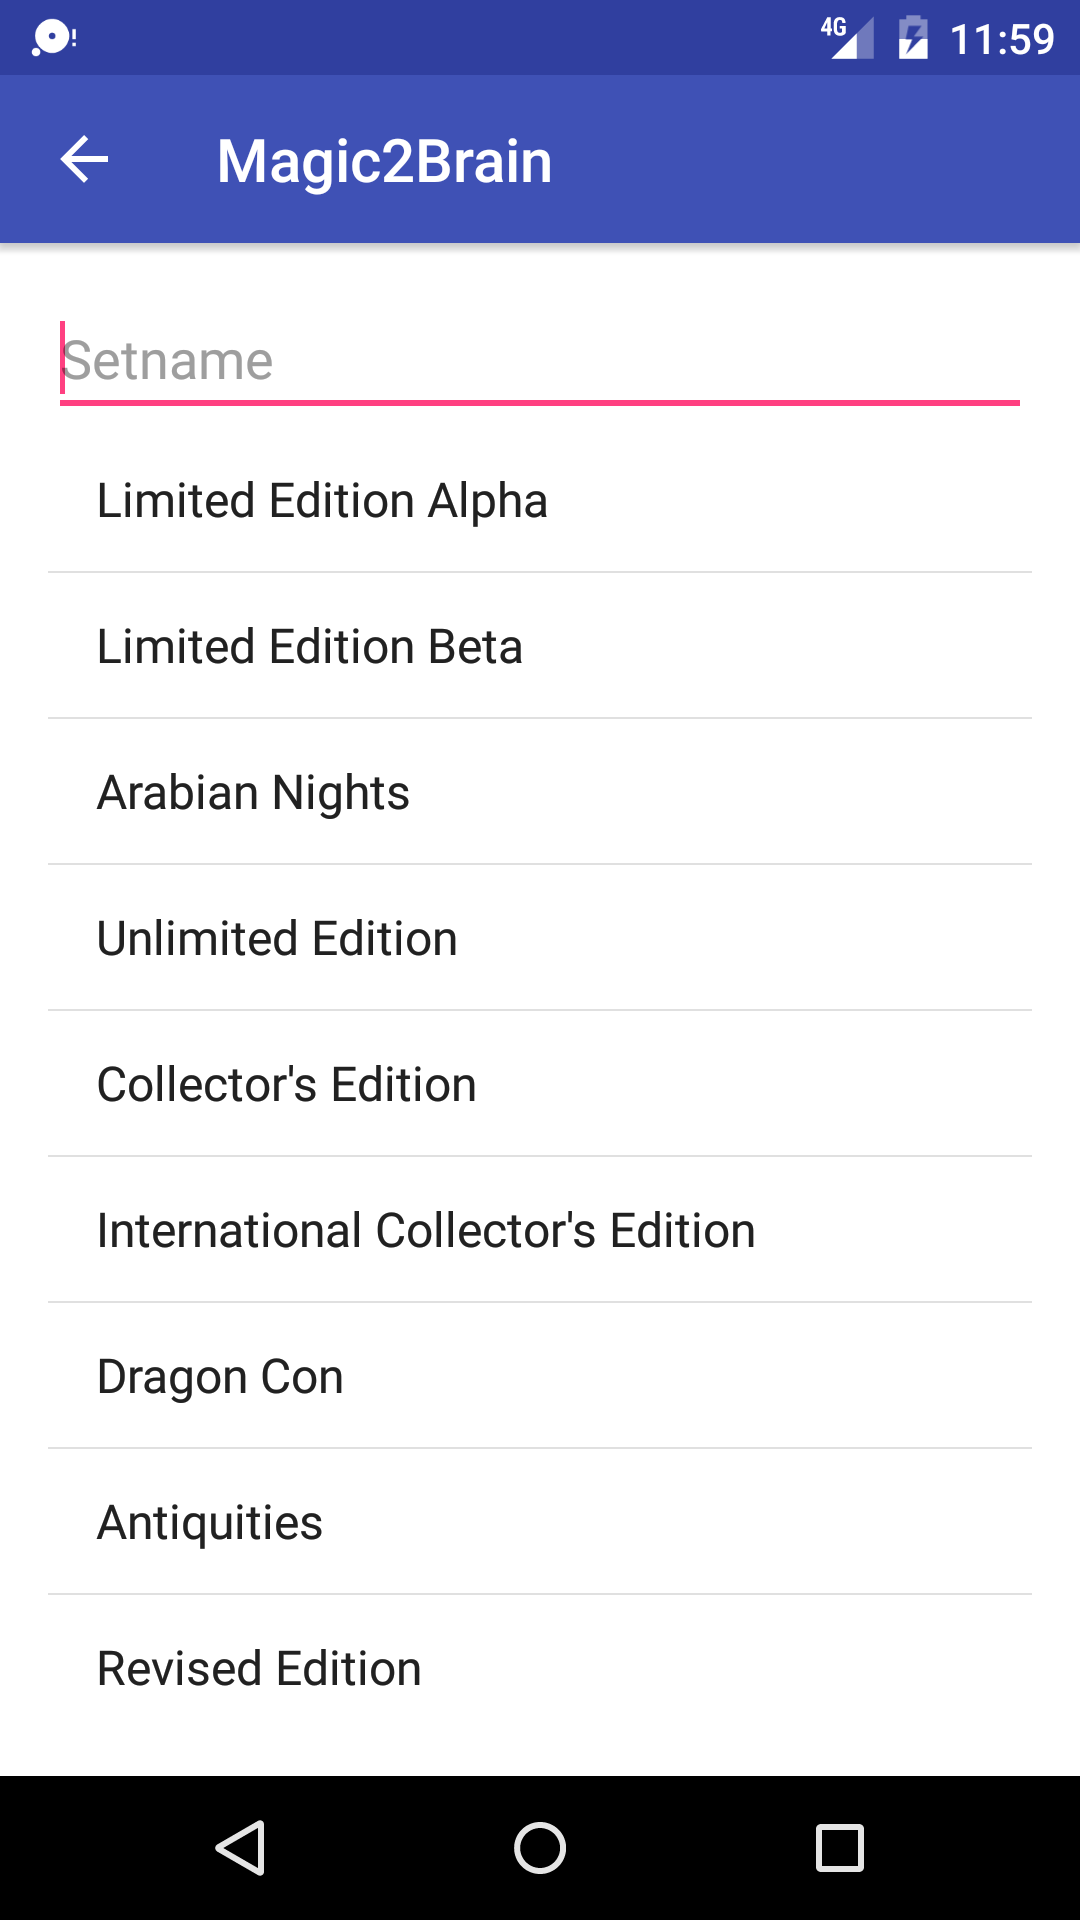
\includegraphics[width=0.3\textwidth]{search.png}
 \caption{Search Activity}
 \label{fig:SearchActivity}
\end{figure}

Dieses Resultat kann entweder mit XML bewerkstelligt werden oder mit Java selber. Im Grunde ist einem diese Entscheidung selber überlassen, da das Wichtigste beim Programmieren persönliche Präferenzen sind.

\subsubsection*{XML}
\begin{lstlisting}
<?xml version="1.0" encoding="utf-8"?>
<RelativeLayout xmlns:android="http://schemas.android.com/apk/res/android"
   xmlns:tools="http://schemas.android.com/tools"
   android:id="@+id/activity_search_handler"
   android:layout_width="match_parent"
   android:layout_height="match_parent"
   android:paddingBottom="@dimen/activity_vertical_margin"
   android:paddingLeft="@dimen/activity_horizontal_margin"
   android:paddingRight="@dimen/activity_horizontal_margin"
   android:paddingTop="@dimen/activity_vertical_margin"
   tools:context="m2b.magic2brain.com.SearchHandlerActivity">

   <EditText
       android:layout_width="wrap_content"
       android:layout_height="wrap_content"
       android:inputType="textPersonName"
       android:ems="10"
       android:id="@+id/search_text"
       android:layout_alignParentTop="true"
       android:layout_alignParentStart="true"
       android:layout_alignParentEnd="true"
       android:contentDescription="Name" />
</RelativeLayout>
\end{lstlisting}

Das Element "`EditText"' ist hier das Texteingabefeld. Im wird mit \verb|android:id=|  eine eindeutige ID zugewiesen, mit der später vom Code aus auf das Element zugegriffen werden kann.
In Java wird das XML folgendermassen eingebunden und auf das Element zugegriffen:
\begin{lstlisting}
//Wichtige imports werden ausgelassen
import m2b.magic2brain.com.magic2brain.R;

//Das Element wird mit der Funktion findViewByID(int ID)
//in der indexierten liste gesucht und gefunden

EditText mTextField = (EditText) findViewByID(R.id.search_text);

//nun kann mit der Variabel mTextField wie gewohnt gearbeitet werden
\end{lstlisting}

\subsubsection*{Java}
Auch bei einer puren Umsetzung in Java ist es nicht ganz möglich dem XML zu entrinnen. Um ein Objekt an ein Layout anzufügen, muss das zuerst verfügbar gemacht werden.
Folglich sieht das XML deutlich kürzer aus, muss aber vorhanden sein. Es muss ausserdem darauf geachtet werden, dem Layout eine ID zu geben, sonst ist es nicht möglich vom Code aus auf das Layout zuzugreifen.
\begin{lstlisting}
<?xml version="1.0" encoding="utf-8"?>
<RelativeLayout xmlns:android="http://schemas.android.com/apk/res/android"
   xmlns:tools="http://schemas.android.com/tools"
   android:id="@+id/activity_search_handler"
   android:layout_width="match_parent"
   android:layout_height="match_parent"
   android:paddingBottom="@dimen/activity_vertical_margin"
   android:paddingLeft="@dimen/activity_horizontal_margin"
   android:paddingRight="@dimen/activity_horizontal_margin"
   android:paddingTop="@dimen/activity_vertical_margin"
   tools:context="m2b.magic2brain.com.SearchHandlerActivity">
</RelativeLayout>
\end{lstlisting}

Wie bereits erwähnt besteht dieses XML nur noch aus dem rohen Layoutblock. \verb|RelativeLayout|  ist eine besondere Art von Layout, die sich hauptsächlich für Apps eignet, die später auf Endgeräten mit verschiedenen Bildschirmgössen vertrieben wird.
Das Einbinden in den Code geschieht wie gewohnt über\\ \verb|findViewByID(R.id.activity_search_handler);| 

\begin{lstlisting}
//Imports werden hier ausgelassen

//Das Layout muss f\"ur die nachfolgenden Schritte gefunden werden
RelativeLayout lyt = (RelativeLayout) findViewById(R.id.activity_search_handler);

//Ein neues, unzugeordnetes Textfeld wird erstellt
EditText mTextField = new EditText(this);

//Nun wird das Textfeld zum Layout hinzugef\"ugt
lyt.addView(mTextField);
\end{lstlisting}

Man sollte XML nur für statische Dinge benutzen, währenddem man Java für dynamische, interaktive Dinge, wie z.B. Bilder oder Textfelder, welche per Knopfdruck hinzugefügt werden können, benutzen sollte.

